\subsubsection{A realistic session: obstacles in mixed order}
\label{sec:res-realworld}

The study ran the obstacles in blocks, but in daily life they come mixed. Each participant's crossings were shuffled 30 times and
the device worked causally: generic model for the first 5 (or 10) crossings, then person scaling learned from the crossings
already walked, without labels (Table~\ref{tab:mixed}, Figure~\ref{fig:realworld}). In mixed order the accuracy grows steadily
from 72\,\% (crossings 1--5) to 79\,\% (6--15) and 90\,\% from crossing 16 on. In the blocked study order the early history
covers only one or two obstacles, the person scaling is biased, and the accuracy collapses for crossings 6--15 before catching up.
The study's blocked-order ``learning during use'' numbers are therefore pessimistic for real use.

\begin{table}[htbp]
\centering
\caption{Accuracy by crossing number in a session, mixed (mean of 30 random orders) vs the real blocked order; generic model until
the switch, then causal person scaling.}
\label{tab:mixed}
\begin{adjustbox}{max width=\textwidth}
{\footnotesize
\begin{tabular}{llrrrrrr}
\toprule
\textbf{order} & \textbf{switch after} & \textbf{crossings 1--5} & \textbf{6--10} & \textbf{11--15} & \textbf{16--20} & \textbf{21+} & \textbf{all} \\
\midrule
mixed & 5 crossings & 71.9\% & 75.1\% & 82.9\% & 87.9\% & 91.3\% & 82.2\% \\
blocked & 5 crossings & 70.0\% & 46.0\% & 56.0\% & 81.2\% & 90.3\% & 69.6\% \\
mixed & 10 crossings & 71.9\% & 73.3\% & 82.9\% & 87.9\% & 91.3\% & 81.9\% \\
blocked & 10 crossings & 70.0\% & 68.0\% & 56.0\% & 81.2\% & 90.3\% & 73.8\% \\
\bottomrule
\end{tabular}
}
\end{adjustbox}

\end{table}

\subsubsection{A virtual real-time cue}
\label{sec:res-cue}

A real-time device must (a) notice the crossing and (b) decide the height while there is still time to cue the trailing limb.
(a) Over all 7250 strides of the sessions, online features available at the foot apex detect 99.0\,\% of the leading-limb
crossing strides, with about 3 false detections per session of about 725 strides. (b) The height is then predicted from the
leading-limb data available at the leading-foot apex (450\,ms before the trailing toe lift-off) or at its landing (200\,ms
before), with causal person scaling (Table~\ref{tab:cue}). In a mixed session about 71\,\% of the crossings get a correct cue at
the apex (76\,\% at landing); after 15 crossings 76\,\% (83\,\%). Answering only above a probability of 0.6 makes 79--82\,\% of
the given cues right but withholds 25--30\,\% of them. The real-time cue is less accurate than the after-the-fact recognition
(about 92\,\%) because only the leading limb has crossed when the cue must be sent.

\begin{table}[htbp]
\centering
\caption{Virtual real-time cue: outcome per crossing (correct / wrong / no cue), share of the given cues that are right, and the
correct cues after 15 crossings. Time left = median time to the trailing toe lift-off.}
\label{tab:cue}
\begin{adjustbox}{max width=\textwidth}
{\scriptsize
\begin{tabular}{lrlrrrrrr}
\toprule
\textbf{cue at} & \textbf{time left} & \textbf{order} & \textbf{threshold} & \textbf{correct cue} & \textbf{wrong cue} & \textbf{no cue (missed or unsure)} & \textbf{cues that are right} & \textbf{correct cue after 15 crossings} \\
\midrule
lead foot apex & 450 ms & mixed & 0.0 & 71.2\% & 27.7\% & 1.2\% & 72.0\% & 76.3\% \\
lead foot apex & 450 ms & mixed & 0.6 & 55.6\% & 14.7\% & 29.8\% & 79.1\% & 63.3\% \\
lead foot apex & 450 ms & blocked & 0.0 & 58.8\% & 40.0\% & 1.2\% & 59.5\% & 75.5\% \\
lead foot apex & 450 ms & blocked & 0.6 & 49.6\% & 23.5\% & 26.9\% & 67.9\% & 65.5\% \\
lead landing & 200 ms & mixed & 0.0 & 75.8\% & 23.1\% & 1.2\% & 76.6\% & 83.2\% \\
lead landing & 200 ms & mixed & 0.6 & 61.2\% & 13.7\% & 25.1\% & 81.7\% & 69.1\% \\
lead landing & 200 ms & blocked & 0.0 & 65.0\% & 33.8\% & 1.2\% & 65.8\% & 80.9\% \\
lead landing & 200 ms & blocked & 0.6 & 54.6\% & 25.0\% & 20.4\% & 68.6\% & 73.6\% \\
\bottomrule
\end{tabular}
}
\end{adjustbox}

\end{table}

\subsubsection{Why some participants are harder}

Once the device is scaled to the person, its errors follow how consistently that person lifts the \emph{trailing} foot for a given
height (Table~\ref{tab:dprime}): the person-scaled accuracy correlates with the trailing-foot separability $d'$ ($r = 0.77$,
leading $d'$: $r = 0.25$). The weakest participant (108, 73\,\%) has by far the least consistent trailing lift ($d' = 0.9$). The
generic model behaves differently ($r = -0.66$ with the trailing $d'$): its errors come from how far a person's personal margin
is from the group, which person scaling removes. With ten participants these correlations are indicative.

\begin{table}[htbp]
\centering
\caption{Per participant: separability of the heights in the leading and trailing foot lift ($d'$), the leading-foot lift SD within
a height and its slope, and the accuracy with person scaling and with the generic model.}
\label{tab:dprime}
\begin{adjustbox}{max width=\textwidth}
{\footnotesize
\begin{tabular}{lrrrrrr}
\toprule
\textbf{participant} & \textbf{lead lift $d'$} & \textbf{trail lift $d'$} & \textbf{lead lift SD within height (mm)} & \textbf{lead slope (mm/cm)} & \textbf{accuracy, person-scaled} & \textbf{accuracy, generic} \\
\midrule
101 & 3.0 & 2.1 & 33 & 11.1 & 94\% & 83\% \\
102 & 2.5 & 2.7 & 45 & 11.2 & 90\% & 63\% \\
103 & 3.7 & 3.6 & 22 & 8.6 & 100\% & 72\% \\
104 & 3.6 & 3.2 & 20 & 8.5 & 96\% & 54\% \\
105 & 4.7 & 2.2 & 19 & 10.2 & 96\% & 84\% \\
106 & 1.2 & 3.4 & 92 & 10.0 & 97\% & 69\% \\
107 & 2.8 & 2.5 & 37 & 10.8 & 85\% & 85\% \\
108 & 2.7 & 0.9 & 29 & 8.8 & 73\% & 85\% \\
109 & 3.5 & 4.5 & 28 & 10.7 & 96\% & 50\% \\
110 & 3.0 & 3.4 & 29 & 10.7 & 96\% & 83\% \\
\bottomrule
\end{tabular}
}
\end{adjustbox}

\end{table}

\begin{figure}[htbp]
\centering
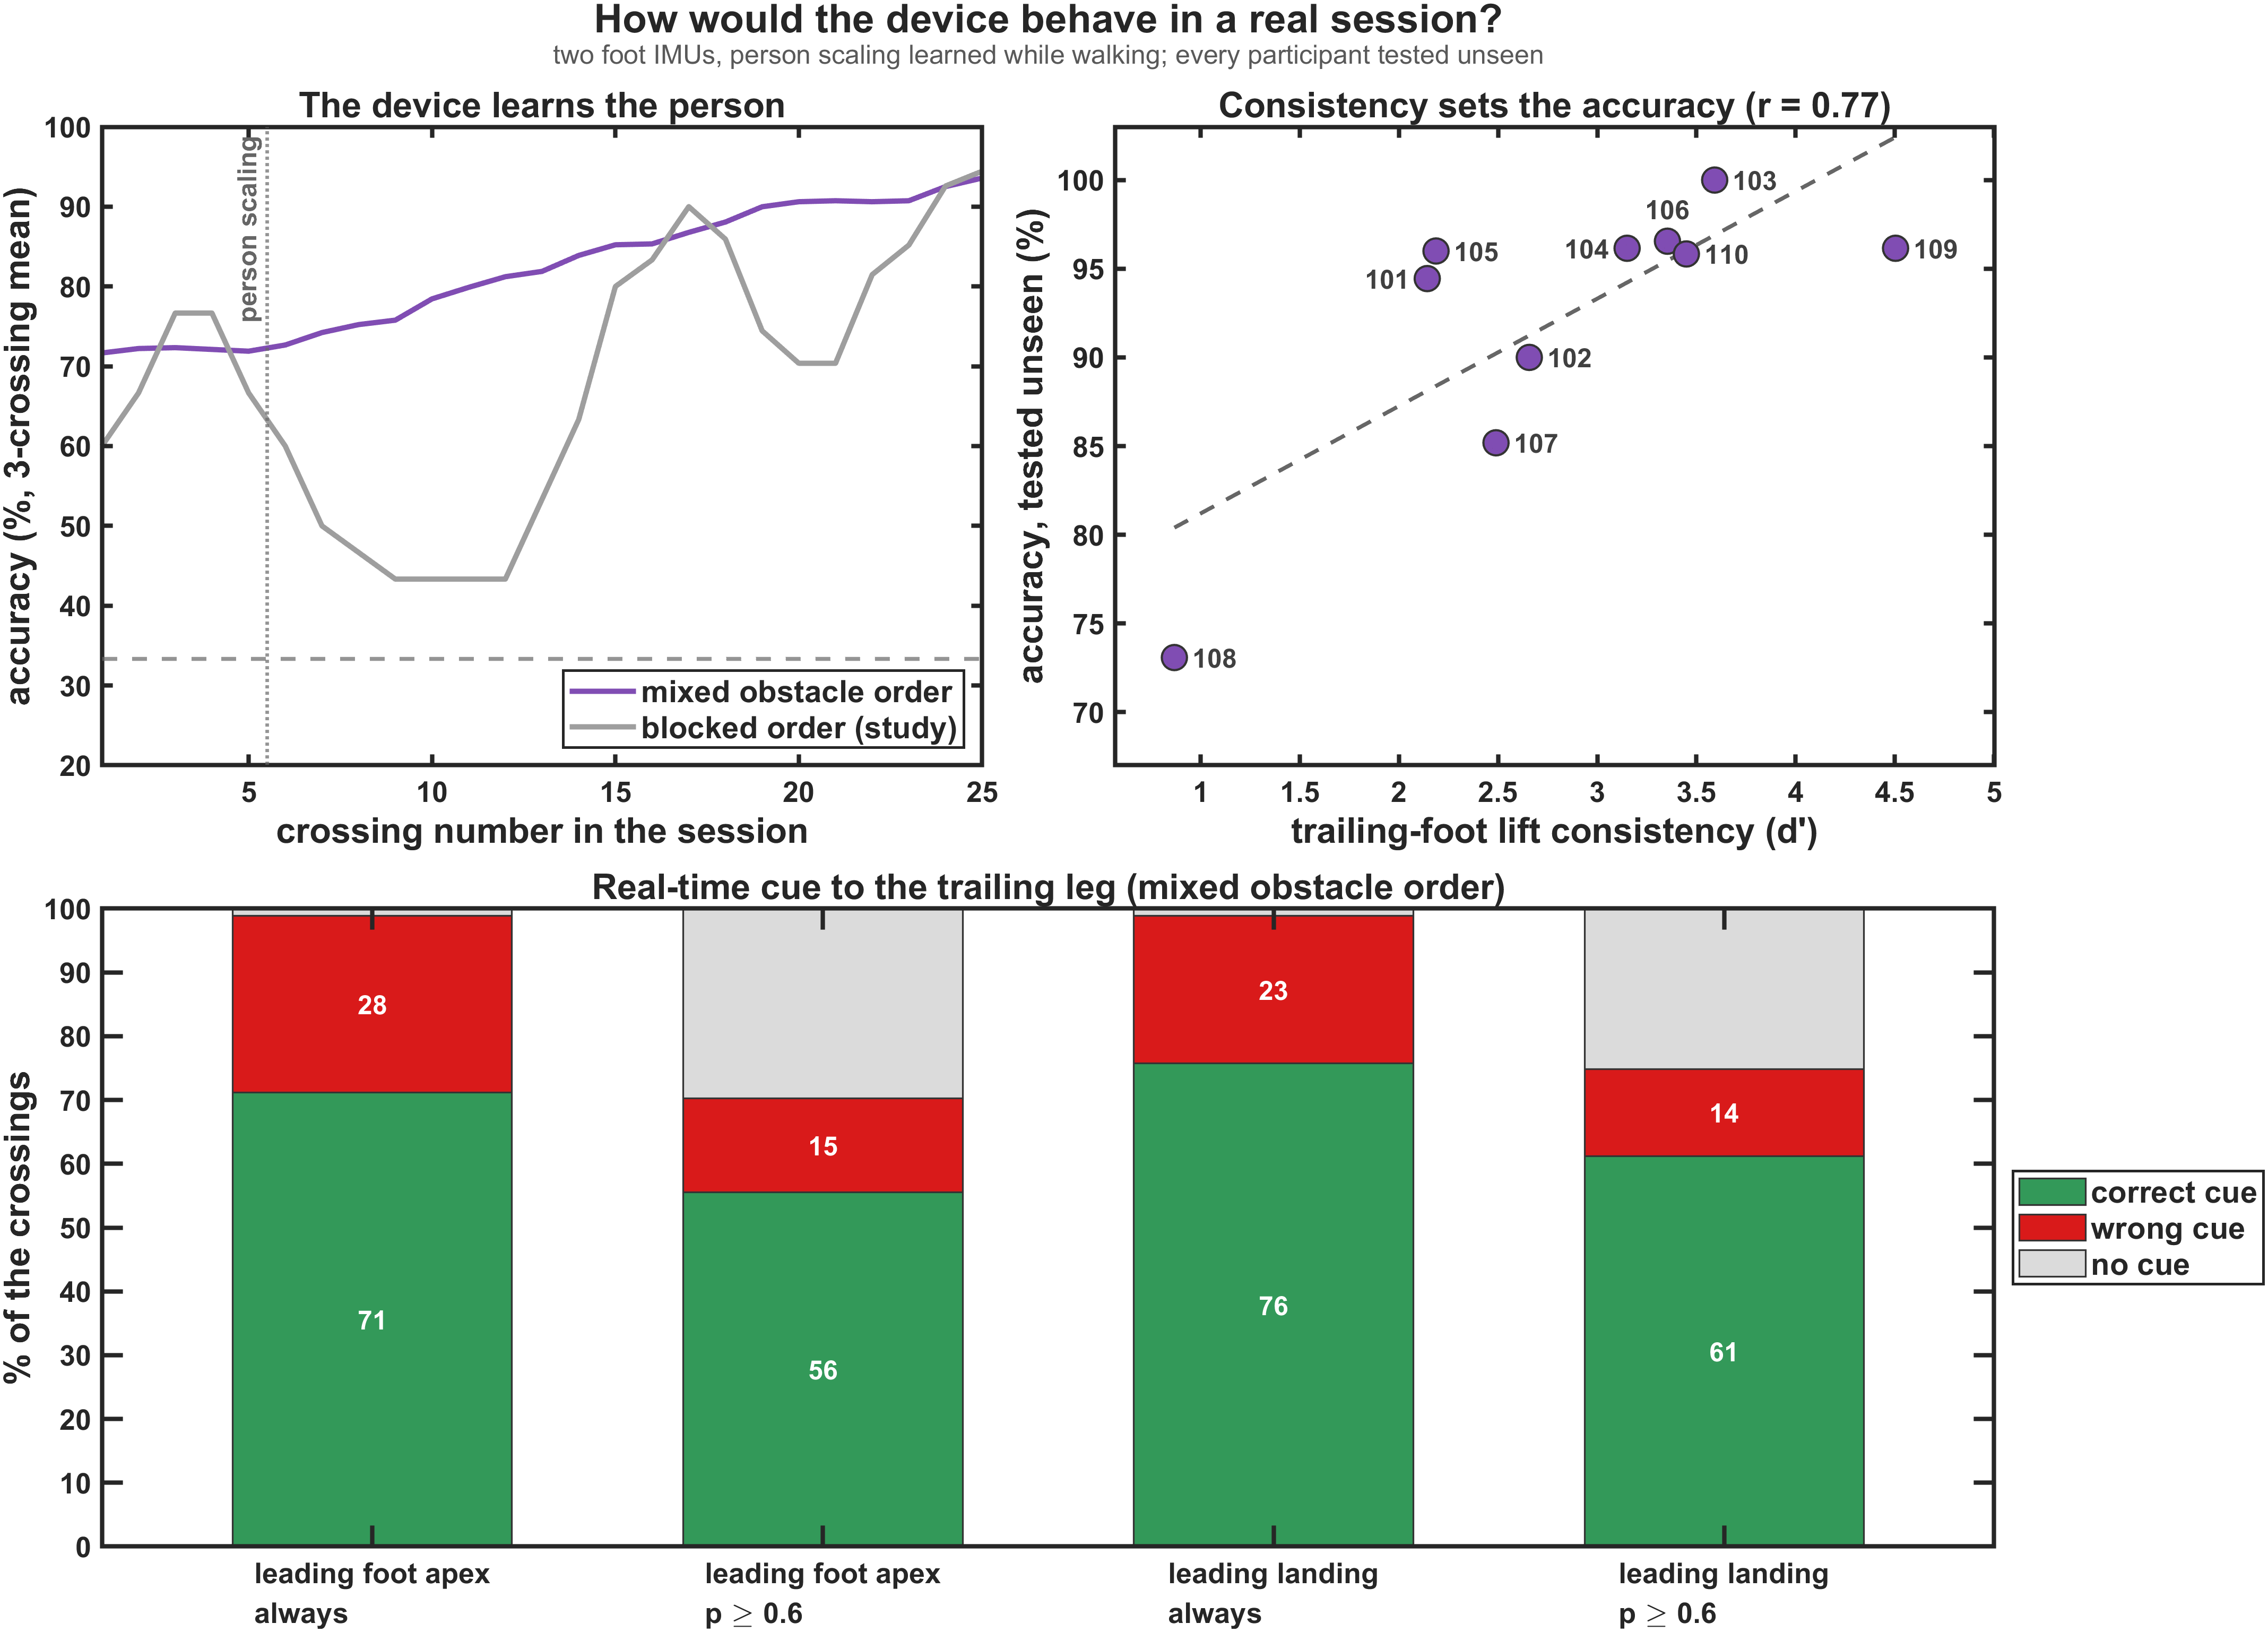
\includegraphics[width=\textwidth]{fig_realworld.png}
\caption{Real-world questions. Top left: accuracy by crossing number in a mixed vs blocked obstacle order (3-crossing moving
mean; dotted = start of person scaling; dashed = chance). Top right: person-scaled accuracy against the trailing-foot separability $d'$ per participant (dashed = least-squares line).
Bottom: outcome of the virtual real-time cue to the trailing leg for each cue moment and confidence threshold (green = correct,
red = wrong, grey = no cue).}
\label{fig:realworld}
\end{figure}
